\begin{figure}[H]
\centering
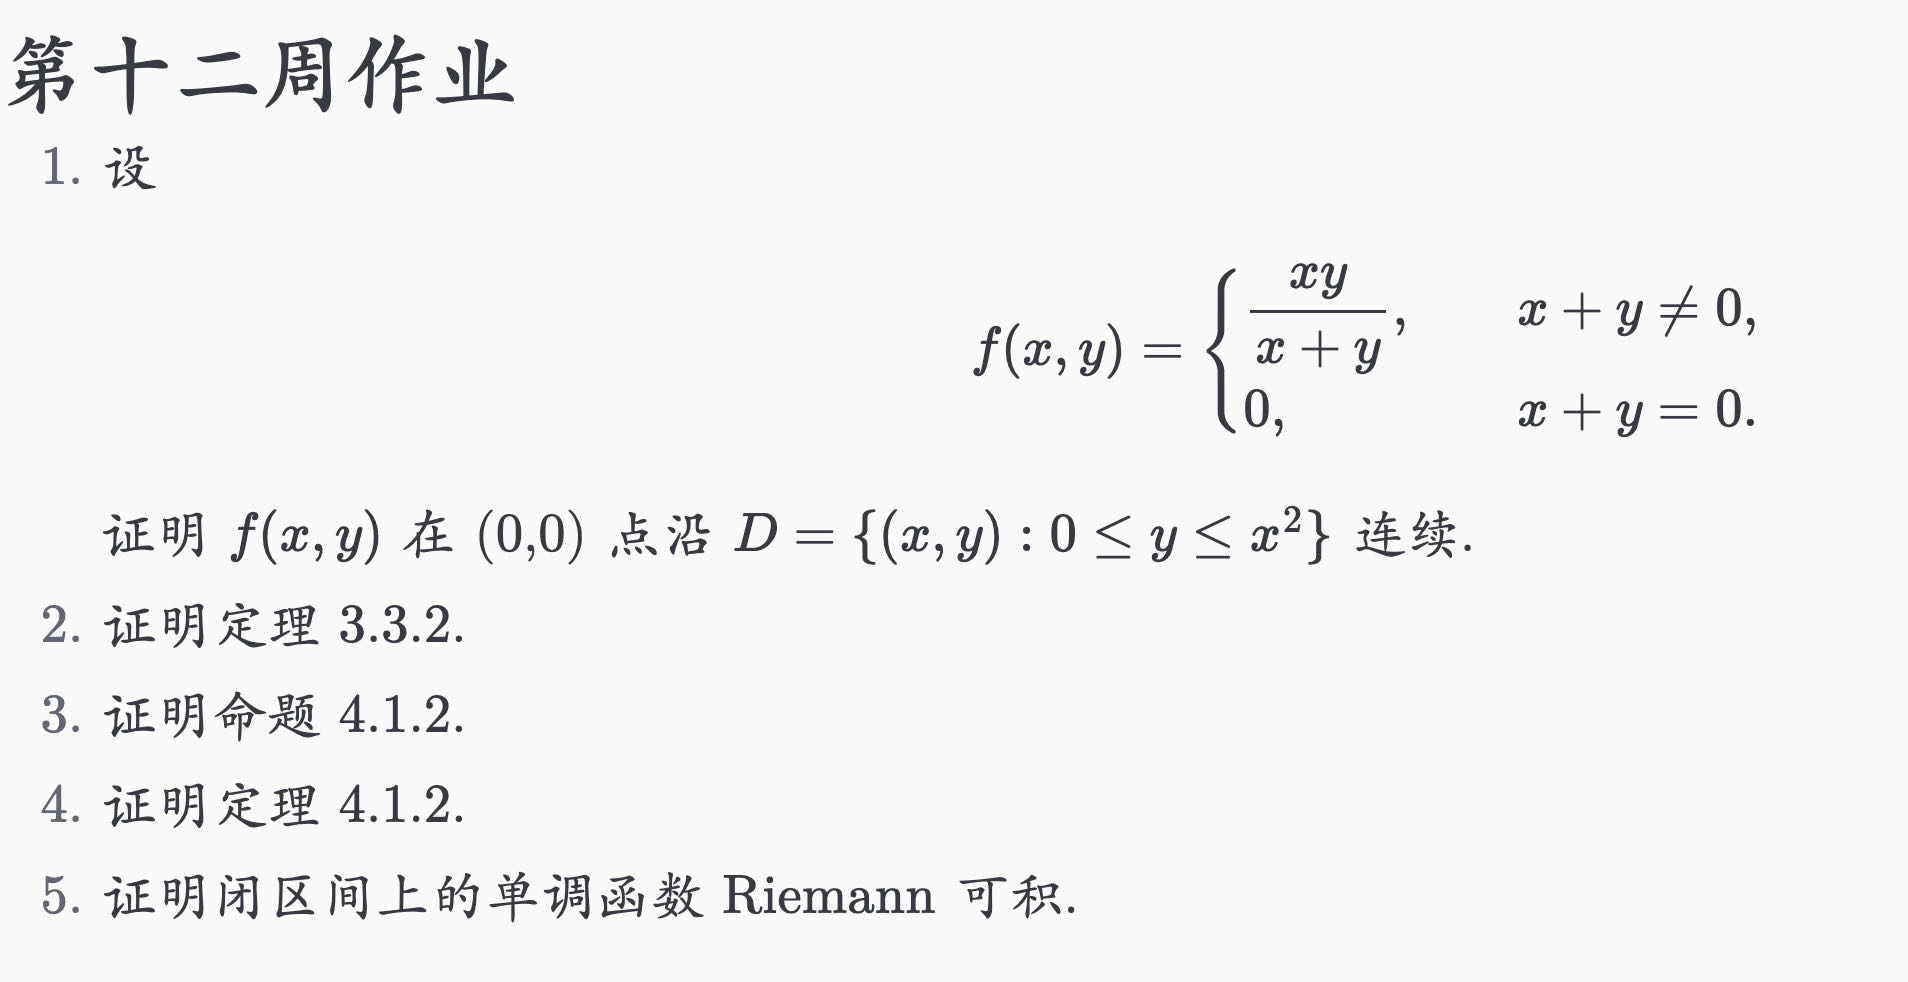
\includegraphics[width=\textwidth]{b3af1a78cc4641ad344199485048bd09.jpg}
% \caption{}
\label{}
\end{figure}

\begin{exercise}
\begin{figure}[H]
\centering
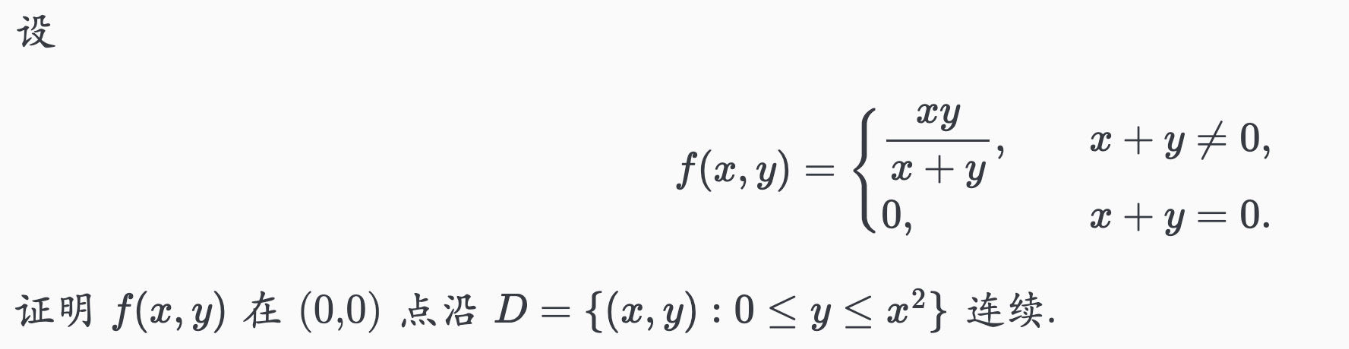
\includegraphics[width=\textwidth]{hw11-2025051923.png}
% \caption{}
\label{}
\end{figure}
\end{exercise}
For $(x, y)\in D$, $\lvert x \rvert<1$, then $y\leq x^2<\lvert x \rvert$, thus $x+y\neq0$,
\[
\lvert f(x,y) \rvert \leq \left\lvert  \frac{xy}{x+y}  \right\rvert \leq \left\lvert  \frac{x\cdot x^2}{x}  \right\rvert =x^2
\]
Let $(x,y)\to0$, then $f(x,y)\to0$, i.e.
\[
\lim_{\substack{(x,y) \to (0,0)\\(x,y)\in D} } f(x,y)=0=f(0,0)
\]
We are done!

\begin{exercise}
\begin{figure}[H]
\centering
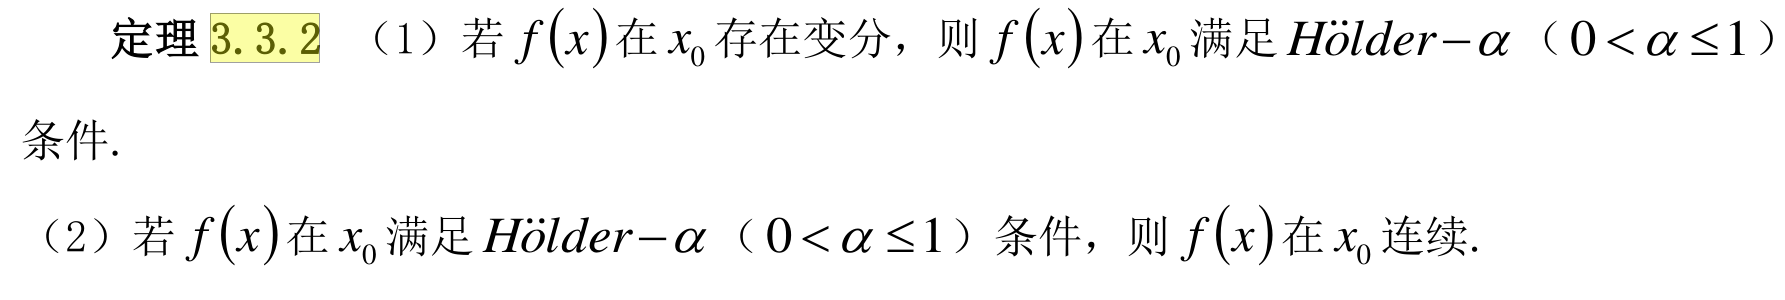
\includegraphics[width=\textwidth]{1-hw11-2025051923.png}
% \caption{}
\label{}
\end{figure}\label{e12f09}
\end{exercise}

(1)
There exists $0<\delta<1$, such that
\[
\lvert f(x_0+\Delta x)-f(x_0)-A_0\Delta x \rvert \leq \lvert \Delta x \rvert
\]
Then for any $\lvert \Delta x \rvert<\delta$
\[
\begin{aligned}
\lvert f(x_0+\Delta x)-f(x_0) \rvert  & \leq \lvert f(x_0+\Delta x)-f(x_0)-A_0\Delta x \rvert +\lvert A_0\Delta x \rvert  \\
 & \leq (1+\lVert A_0 \rVert )\lvert \Delta x \rvert  \\
 & \leq (1+\lVert A_0 \rVert )\lvert \Delta x \rvert ^{\alpha}\qquad \forall \alpha\in(0,1]
\end{aligned}
\]
where $\lVert A_0 \rVert=\sup_{\lvert x \rvert=1}\frac{\lvert A_0x \rvert}{\lvert x \rvert}$.

(2)
If
\[
\lvert f(x_0+\Delta x)-f(x_0) \rvert \leq C_{\alpha}\lvert \Delta x \rvert ^{\alpha}
\]
for some $\alpha\in(0,1]$. Let $\lvert \Delta x \rvert\to0$, then $\lvert f(x_0+\Delta x)-f(x_0) \rvert\to0$. Thus $f$ is continuous at $x_0$.

\begin{definition}[变分]
\begin{figure}[H]
\centering
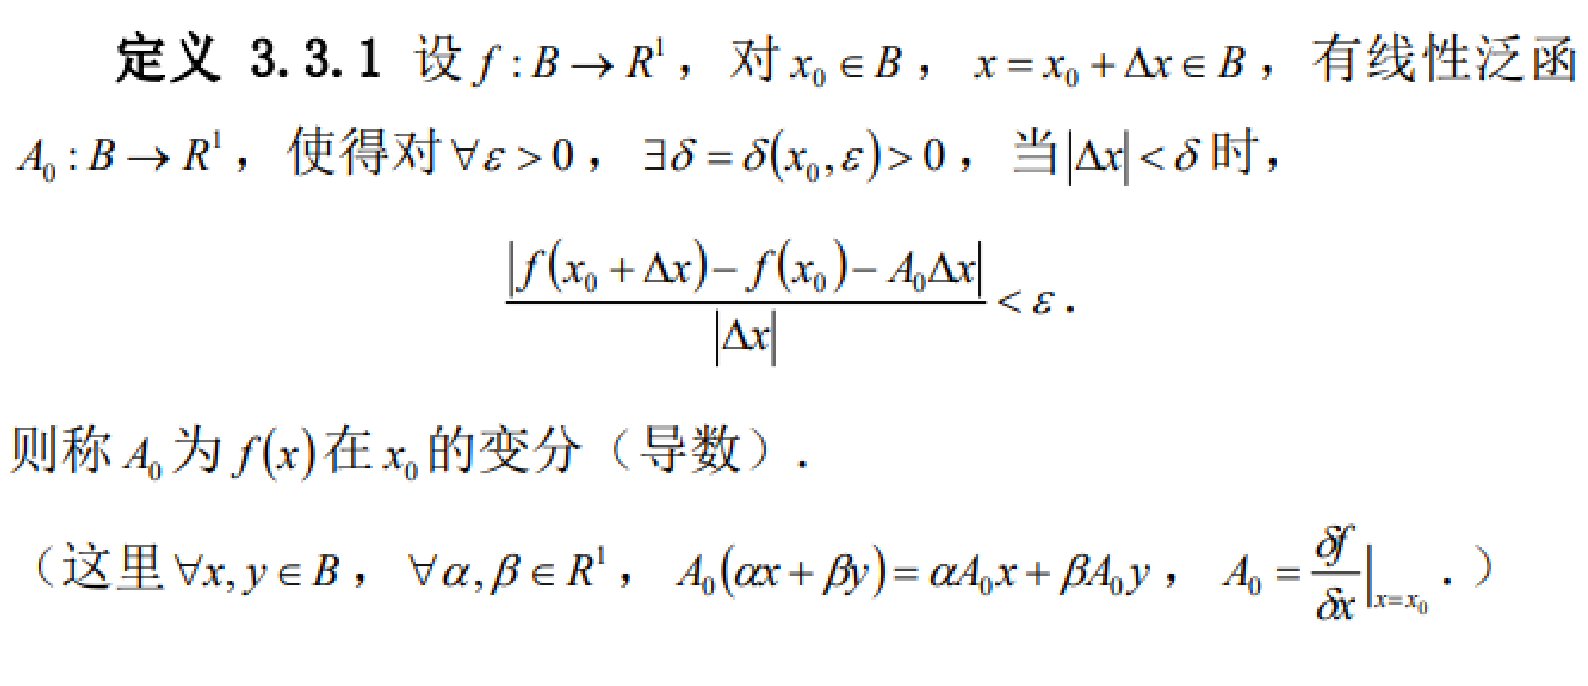
\includegraphics[width=\textwidth]{2-hw11-2025051923.png}
% \caption{}
\label{}
\end{figure}
\end{definition}
\begin{definition}[Holder 条件]
\begin{figure}[H]
\centering
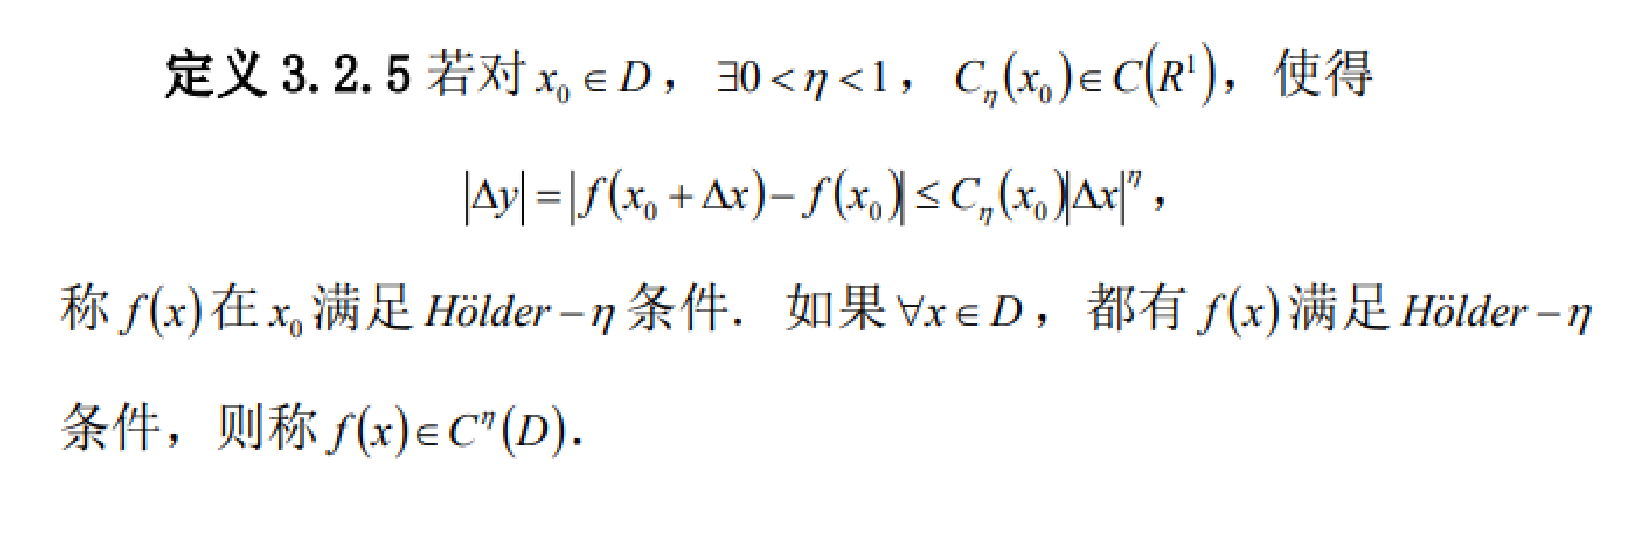
\includegraphics[width=\textwidth]{3-hw11-2025051923.png}
% \caption{}
\label{}
\end{figure}\label{ddc2af}
\end{definition}

\begin{exercise}
\begin{figure}[H]
\centering
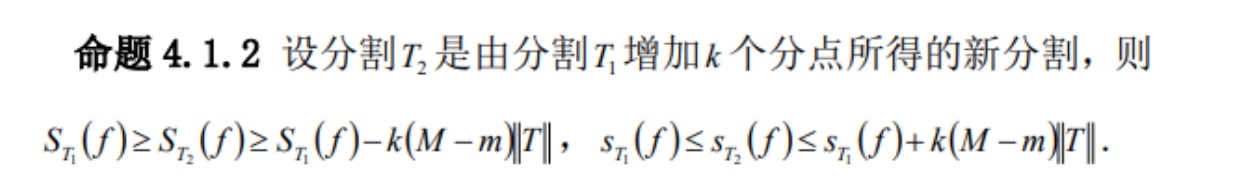
\includegraphics[width=\textwidth]{hw11-2025052000.png}
% \caption{}
\label{}
\end{figure}
\end{exercise}
\begin{proof}
由于将 $k$ 个分点一次插入 $T_1$ 与将这 $k$ 个分点逐个插入 $T_1$,所得到的都是分割 $T_2$,因此我们可以考虑将这 $k$ 个分点逐个插入 $T_1$ 的情况。设步长为 $\|T\|$.

设
\[
T_1 = \{x_i\}_{i=0}^n, \quad a = x_0 < x_1 < \cdots < x_{n-1} < x_n = b.
\]
先考虑在 $T_1$ 中插入一个分点 $x'_i$,记对应的新分割为 $T_1'$,不妨设 $x'_i$ 被插入小区间 $[x_{i-1}, x_i]$ 中,于是
\[
T_1': a = x_0 < x_1 < \cdots < x_{i-1} < x'_i < x_i < \cdots < x_{n-1} < x_n = b.
\]
这样,对应于分割 $T_1'$ 的小区间有 $n+1$ 个,它们包含分割 $T_1$ 的 $n-1$ 个完全相同的小区间以及 $[x_{i-1}, x_i]$ 被 $x'_i$ 分成的两个子区间 $[x_{i-1}, x'_i]$, $[x'_i, x_i]$. 记
\[
M'_i = \sup_{x \in [x_{i-1}, x'_i]} \{f(x)\}, \quad M''_i = \sup_{x \in [x'_i, x_i]} \{f(x)\}, \quad \Delta x'_i = x'_i - x_{i-1}, \quad \Delta x''_i = x_i - x'_i.
\]
则
\[
\begin{aligned}
S_{T_1'}(f) - S_{T_1}(f) &= M_i \Delta x_i - (M'_i \Delta x'_i + M''_i \Delta x''_i)  \\
 & = M_i (\Delta x'_i + \Delta x''_i) - (M'_i \Delta x'_i + M''_i \Delta x''_i) \\
&= (M_i - M'_i) \Delta x'_i + (M_i - M''_i) \Delta x''_i
\end{aligned}
\]
由于
\[
0 \leq (M_i - M'_i) \Delta x'_i + (M_i - M''_i) \Delta x''_i \leq (M - m) \Delta x'_i + (M - m) \Delta x''_i = (M - m) \Delta x_i \leq (M - m) \|T\|
\]
所以 $S_{T_1}(f) - S_{T_1'}(f) \leq (M-m)\|T\|$, 即 $S_{T_1'}(f) \geq S_{T_1}(f) - (M-m)\|T\|$. 从而有
\[
S_{T_1}(f) \geq S_{T_1'}(f) \geq S_{T_1}(f) - (M-m)\|T\|.
\]
对于在 $T_1$ 中插入两个分点对应的分割 $T_1^2$,可以看成在 $T_1'$ 中插入一个分点,于是有 $S_{T_1}(f) \geq S_{T_1^2}(f)$, 且 $S_{T_1'}(f) - S_{T_1^2}(f) \leq (M-m)\|T\|$. 从而
\[
S_{T_1}(f) \geq S_{T_1^2}(f) \geq S_{T_1'}(f) - (M-m)\|T\| \geq S_{T_1}(f) - (M-m)\|T\| - (M-m)\|T\| = S_{T_1}(f) - 2(M-m)\|T\|.
\]
分割 $T_2$ 是由分割 $T_1$ 增加 $k$ 个分点所得的新分割,则
\[
S_{T_1}(f) \geq S_{T_2}(f) \geq S_{T_1}(f) - k(M-m)\|T\|.
\]
对于不等式的第二部分 $s_{T_2}(f) \leq s_{T_1}(f) + k(M-m)\|T_1\|$: 当从 $T^{(j-1)}$ 添加一个分点得到 $T^{(j)}$ 时,这个新分点必然落入 $T^{(j-1)}$ 的某个子区间,设其长度为 $\delta_j$。根据单点插入的结果,我们有: $s_{T^{(j)}}(f) \leq s_{T^{(j-1)}}(f) + (M - m) \delta_j$. 由于 $T^{(j-1)}$ 是 $T_1$ 的一个加细分割(或者是 $T_1$ 本身),其任何子区间的长度 $\delta_j$ 都不会超过 $T_1$ 的最大子区间长度,即 $\delta_j \leq \|T_1\|$。所以, $s_{T^{(j)}}(f) \leq s_{T^{(j-1)}}(f) + (M - m) \|T_1\|$ 对于 $j = 1, 2, \dots, k$。现在我们可以进行迭代:
\[
\begin{aligned} s_{T_2}(f) = s_{T^{(k)}}(f) &\leq s_{T^{(k-1)}}(f) + (M - m) \|T_1\| \\ &\leq (s_{T^{(k-2)}}(f) + (M - m) \|T_1\|) + (M - m) \|T_1\| \\ &= s_{T^{(k-2)}}(f) + 2(M - m) \|T_1\| \\ &\vdots \\ &\leq s_{T^{(0)}}(f) + k(M - m) \|T_1\| \\ &= s_{T_1}(f) + k(M - m) \|T_1\|. \end{aligned}
\]
这就证明了不等式的第二部分:$s_{T_2}(f) \leq s_{T_1}(f) + k(M-m)\|T_1\|$。 综上所述,对于下和,我们已经完整证明了: \[
s_{T_1}(f) \leq s_{T_2}(f) \leq s_{T_1}(f) + k(M-m)\|T_1\|.
\] 命题证毕。

\end{proof}

\begin{exercise}
\begin{figure}[H]
\centering
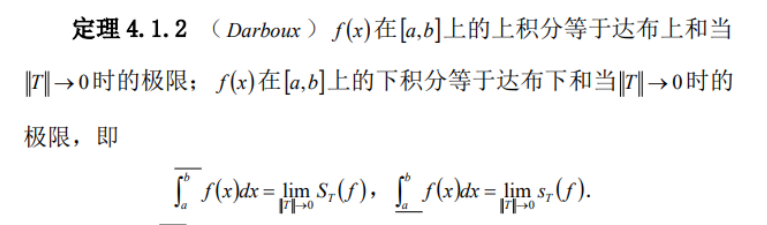
\includegraphics[width=\textwidth]{1-hw11-2025052000.png}
% \caption{}
\label{}
\end{figure}
\end{exercise}
只需要证明
\[
\inf \{ S_{P}(f)\mid P \text{ 是 } [a, b] \text{ 的一个划分} \}=\lim_{ \lVert T \rVert  \to 0 } S_{T}(f)
\]
对于任意给定的 $[a,b]$ 的划分 $T$, 由定义可知
\[
\inf \{ S_{P}(f)\mid P \text{ 是 } [a, b] \text{ 的一个划分} \}\leq S_{T}(f)
\]
令 $\lVert T \rVert\to0$ 就有
\[
\inf \{ S_{P}(f)\mid P \text{ 是 } [a, b] \text{ 的一个划分} \}\leq \lim_{ \lVert T \rVert  \to 0 } S_{T}(f)
\]
另一方面,对于任意给定的 $[a,b]$ 的划分 $P$, 由 \cref{e12f09},
\[
S_{P}(f)\geq S_{T\cup P}(f)\geq S_{T}(f)-(n-1)(M-m)\lVert T \rVert 
\]
令 $\lVert T \rVert\to0$ 就有
\[
S_{P}(f)\geq \lim_{ \lVert T \rVert  \to 0 } S_{T}(f)
\]
再对 $P$ 取 $\inf$ 就有
\[
\inf \{ S_{P}(f)\mid P \text{ 是 } [a, b] \text{ 的一个划分} \}\geq  \lim_{ \lVert T \rVert  \to 0 } S_{T}(f)
\]
故
\[
\overline{\int_a^b} f(x) \, dx=\inf \{ S_{P}(f)\mid P \text{ 是 } [a, b] \text{ 的一个划分} \}= \lim_{ \lVert T \rVert  \to 0 } S_{T}(f)
\]
类似可证:
\[
\underline{\int_a^b} f(x) \, dx =\sup \{ s_{P}(f)\mid P \text{ 是 } [a, b] \text{ 的一个划分} \}= \lim_{ \lVert T \rVert  \to 0 } s_{T}(f)
\]
\begin{definition}[上积分的定义]
设 $f: [a, b] \to \mathbb{R}$ 是一个有界函数。对于 $[a, b]$ 的一个划分 $P = \{x_0, x_1, \dots, x_n\}$,其中 $a = x_0 < x_1 < \dots < x_n = b$,令 $M_i = \sup \{ f(x) \mid x \in [x_{i-1}, x_i] \}$。上达布和定义为 $U(f, P) = \sum_{i=1}^n M_i (x_i - x_{i-1})$。
\textbf{上积分} $\overline{\int_a^b} f(x) \, dx$ 定义为所有上达布和的下确界:
\[
\overline{\int_a^b} f(x) \, dx = \inf \{ U(f, P) \mid P \text{ 是 } [a, b] \text{ 的一个划分} \}
\]
\end{definition}
\begin{definition}[下积分的定义]
设 $f: [a, b] \to \mathbb{R}$ 是一个有界函数。对于 $[a, b]$ 的一个划分 $P = \{x_0, x_1, \dots, x_n\}$,其中 $a = x_0 < x_1 < \dots < x_n = b$,令 $m_i = \inf \{ f(x) \mid x \in [x_{i-1}, x_i] \}$。下达布和定义为 $L(f, P) = \sum_{i=1}^n m_i (x_i - x_{i-1})$。
\textbf{下积分} $\underline{\int_a^b} f(x) \, dx$ 定义为所有下达布和的上确界:
\[
\underline{\int_a^b} f(x) \, dx = \sup \{ L(f, P) \mid P \text{ 是 } [a, b] \text{ 的一个划分} \}
\]
\end{definition}
\begin{definition}[Darboux 上和与下和]
设 $f$ 是定义在 $[a,b]$ 上的有界函数, $P$ 是 $[a,b]$ 的一个分割. 记 $M_i = \sup_{x \in [x_{i-1}, x_i]} f(x)$ 和 $m_i = \inf_{x \in [x_{i-1}, x_i]} f(x)$. 定义 $f$ 关于分割 $P$ 的 \textbf{Darboux 上和} 为
\[
U(f,P) = \sum_{i=1}^n M_i (x_i - x_{i-1})
\]定义 $f$ 关于分割 $P$ 的 \textbf{Darboux 下和} 为
\[
L(f,P) = \sum_{i=1}^n m_i (x_i - x_{i-1})
\]
\end{definition}
\begin{exercise}
\begin{figure}[H]
\centering

\includegraphics[width=\textwidth]{2-hw11-2025052000.png}
% \caption{}
\label{}
\end{figure}
\end{exercise}
\begin{note}
由于闭区间单调函数有界,单调函数间断点至多可数,由 Lebesgue 定理可知,闭区间单调函数 Riemann 可积.
\end{note}
\begin{theorem}[Lebesgue 定理]
$f:[a, b] \rightarrow \mathbb{R}$ 是有界的. 则 $f$ 黎曼可积当且仅当 $f$ 的不连续点集是勒贝格零测集.
\end{theorem}
下面我们给出一个初等的证明:

\begin{figure}[H]
\centering
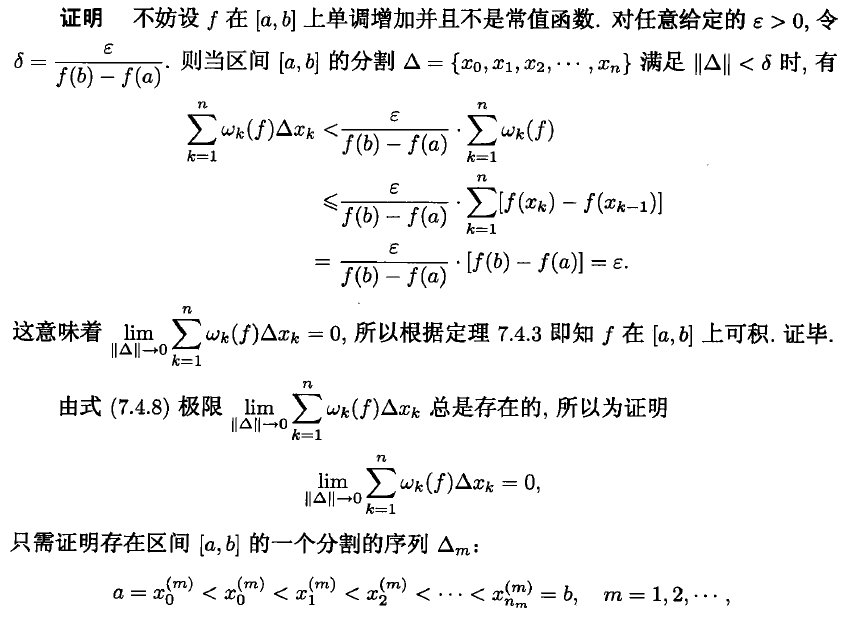
\includegraphics[width=\textwidth]{hw11-2025052001.png}
% \caption{}
\label{}
\end{figure}
\begin{figure}[H]
\centering
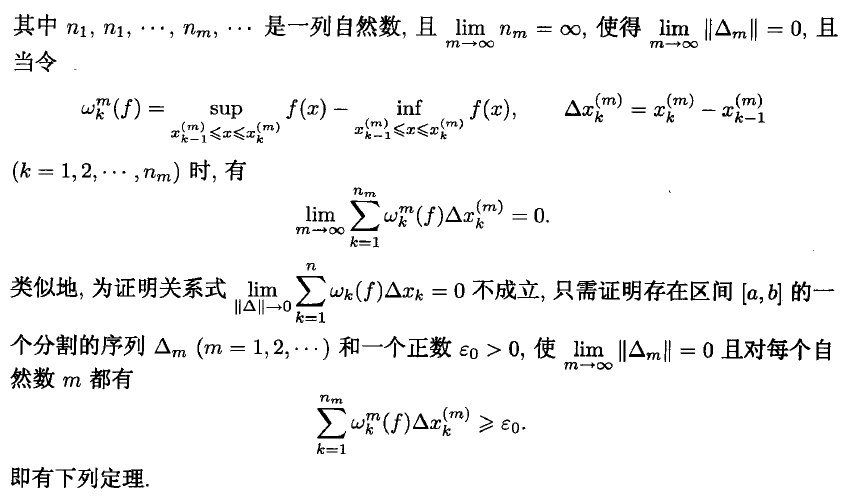
\includegraphics[width=\textwidth]{1-hw11-2025052001.png}
% \caption{}
\label{}
\end{figure}

\begin{figure}[H]
\centering
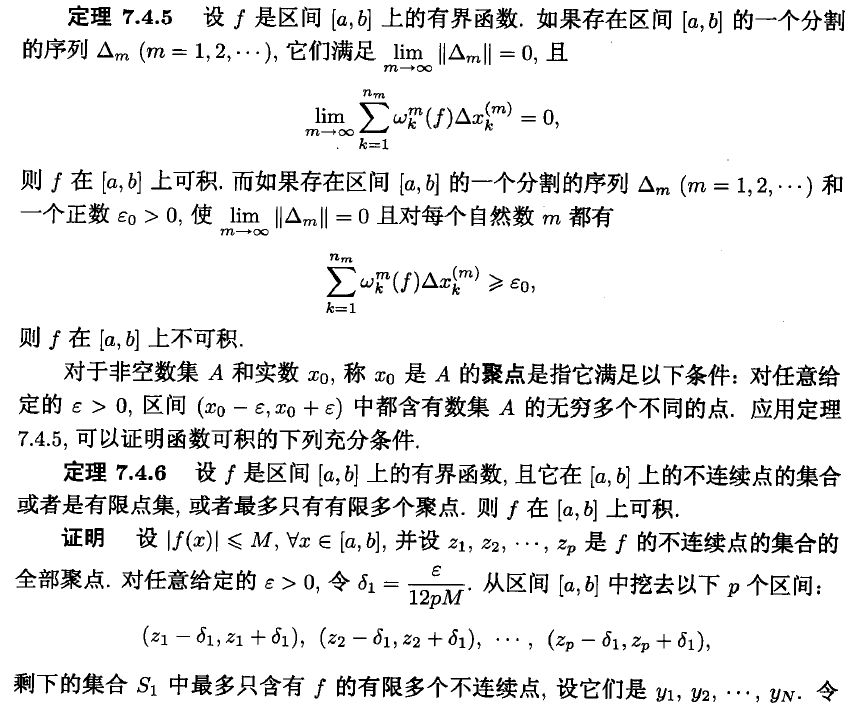
\includegraphics[width=\textwidth]{2-hw11-2025052001.png}
% \caption{}
\label{}
\end{figure}
\begin{figure}[H]
\centering
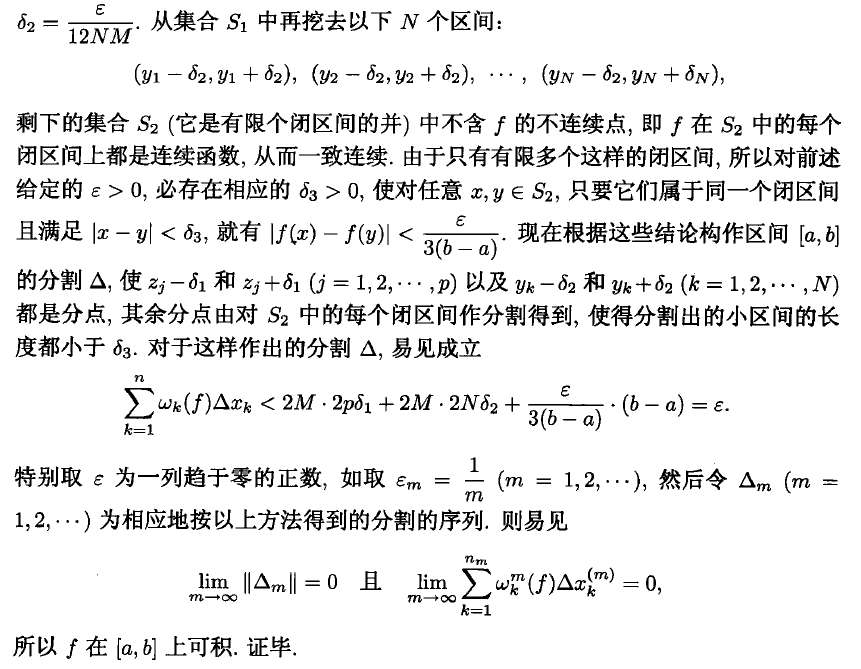
\includegraphics[width=\textwidth]{3-hw11-2025052001.png}
% \caption{}
\label{}
\end{figure}
